% Chapter 1

\chapter{Dissertation Overview} % Main chapter title

\label{overview} % For referencing the chapter elsewhere, use \ref{Chapter1} 

\lhead{Chapter 1. \emph{Dissertation Overview}} % This is for the header on each page - perhaps a shortened title

%\section{Social Media and Real-life Events}
% It has provided a communication platform to the masses enabling them to post short real-time messages in the form of micro-blogs, status updates, photographs and videos, to write full length articles expressing their views in blogs. This has turned the information consumers to original information producers and curators. According to a recent survey reported by Pew Research about 46\% of adult Internet users post original photos or videos online that they themselves have created \cite{pewresearch}. The humungous volumes of dynamic user-generated real-time data from social media provide great opportunities to businesses, governments, and researchers to tap valuable meaningful information for further analysis.

Social media is a paradigm shift in the way people communicate with each other. It has grown from being just a medium to a global medium of communication between people. Different types of social media platforms provide multiple venues for people to share firsthand experiences and exchange information about real-life events. It has become an indispensable means for disseminating news and real-time information about current events, using websites such as Twitter, Facebook, Instagram, Flickr, Youtube, Google Plus and Vine. These applications allow users to post short textual messages accompanied by images and videos. At the same time users also share their detailed journalistic experiences in the form of diaries through blogging platforms such as Blogger, Wordpress and Medium. Studies have shown the importance of social media platforms as a news circulation service \cite{phelan2009using}, and a source for gauging public interest and opinions \cite{o2010tweets,singh2010clustering,singh2010mining,agarwal2012online}. Its efficacy as a real-time, citizen-journalistic source of information has been recently harnessed in the detection, extraction and analysis of real-life events \cite{sakaki2013tweet,popescu2011extracting,purohit2013twitris}. The activities of users producing content in social media has also been studied for gaining deep insights about how users form communities around topics related to real-life events \cite{agarwal2013grouping,agarwal2014time,sen2012identifying} that lead to collective action \cite{agarwal2014online,agarwal2012raising}.

With the popularity of social media there has been proliferation of unstructured textual content on the Internet about different real-life events. Tracking social media for useful content such as live reporting of an event and recent updates can be harnessed to identify important nuggets of information. It can lead to identification and analysis of insightful user-generated information about named entities (people, place, organization, etc). Event summaries can be generated from the identified event-specific informative content. Actionable event-specific insights can be extracted such as, ``what is happening", ``who is involved", ``where is it happening", ``when did it happen", and so on. There are tremendous applications in the areas of real-life event analysis, data journalism, event management, opinion mining, online targeted marketing, cyber security, among others. Thus, there is a need of a generic framework that has the following capabilities:
\begin{itemize}
\item Collecting different types of textual content produced in social media related to an event.
\item Extracting information that acts as an identity of the event used for characterizing it
\item Maintaining the extracted event identity information persistently for resolving constantly produced new content and discovering important event-specific information. 
\end{itemize}


The problem of collecting and extracting event identity information from social media is very similar to the task of event detection and tracking from newswires \cite{allan1998line,kumaran2004text}. However, in this dissertation, we add new components that creates persistent identity structures of an event and update it with new information over time. In order to make our task well-defined we focus on the problem of tracking a pre-specified set of events. Also, the domain of social media poses additional challenges. News articles most often adhere to grammatical, syntactical and formal structures of writing, that are not common in the realm of social media. The user-generated content in social media is most often colloquial, short, noisy, and lacks proper grammatical structure. This makes it a challenging task for even the state-of-the-art natural language processing techniques to extract useful information and to perform tasks like entity extraction and parts-of-speech tagging that lies at the core of the previous research on event detection and tracking.

The work presented in this dissertation establishes the conceptual design and implementation of a framework capable of collecting, extracting and persistently managing event identity information from user-generated short textual content shared in social media (shown in Figure 1.1). The approach of the presented work is from the perspective of Entity Identity Information Management (EIIM) \cite{zhou2011entity}, with basic tenets of information quality at its core. Towards this objective, different challenges of mining high quality information from social media text is discussed and a patent-pending, novel approach to the challenges of identifying event-specific informative content is explained. This approach is a critical component of the framework. The dissertation further explores the applications of the research and concludes by discussing future directions of the work.


%The thesis introduces the problem of Event Identity Information Management in social media, discusses the prevalent challenges and presents the implementation design of a framework capable of managing persistent identity information of pre-specified set of real-life events. It further explores the applications of the research and concludes by pointing to different future directions of the work. 

\begin{figure}[htbp]
\label{eiim}
  \caption{Event Identity Information Management (EIIM) Life Cycle for user generated textual content in social media}
  \centering
    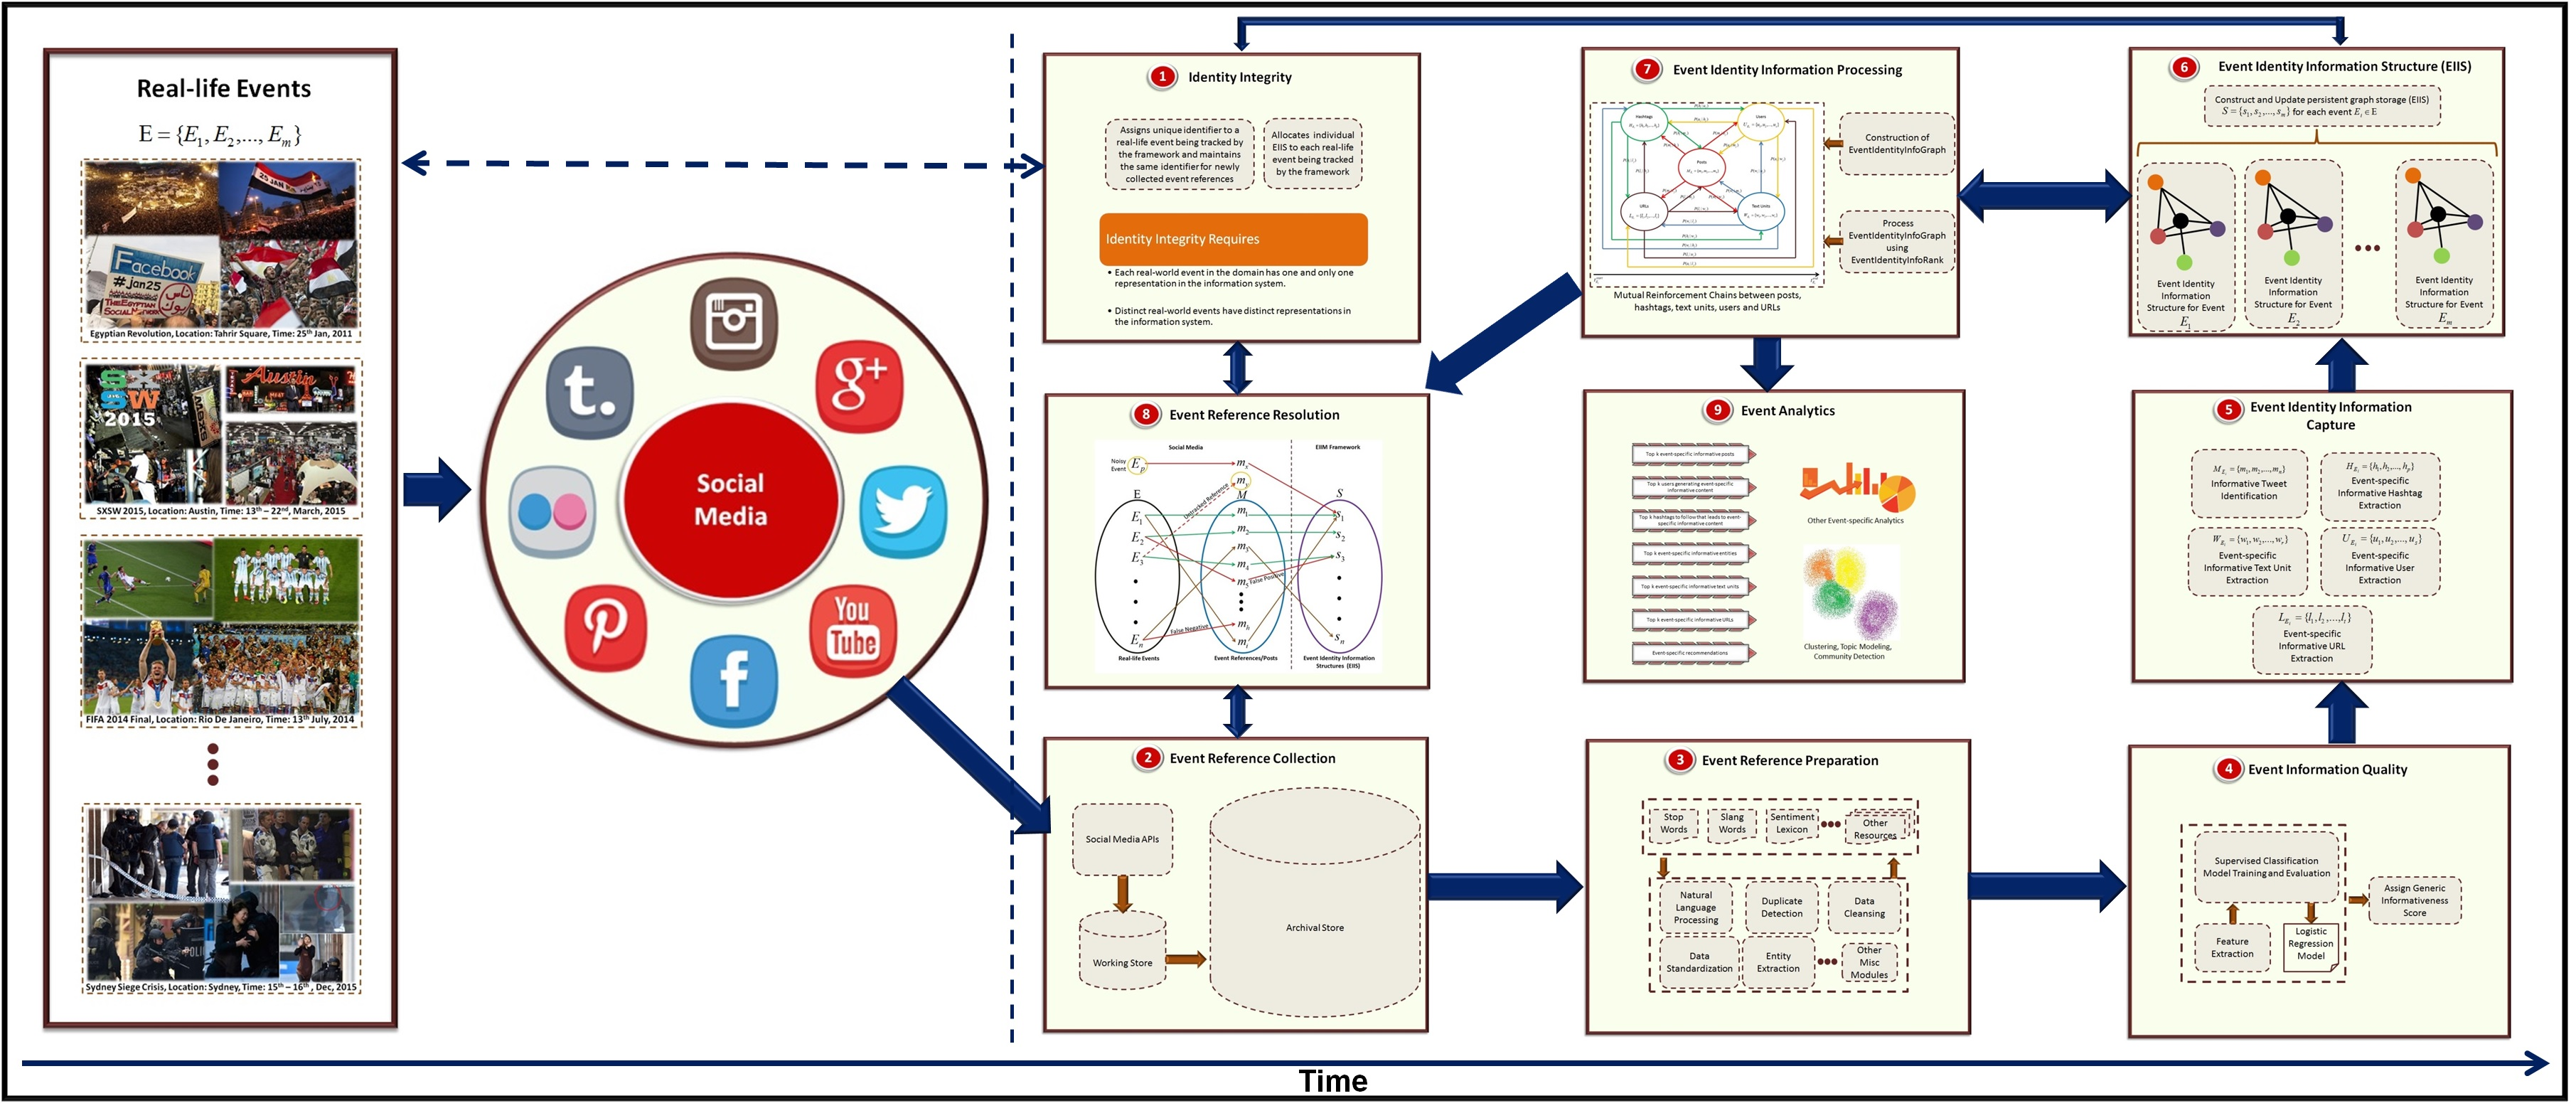
\includegraphics[width=15.5cm,height=7cm]{Figures/EIIM.jpg}
\end{figure}

Some of the main contributions of the work are:

\begin{itemize}
\item Extending the Entity Identity Information Management (EIIM) model  \cite{zhou2011entity} from the closed world domain of Master Data Management (MDM) to the open and unstructured domain of social media.

\item The design and implementation of an \textit{Event Identity Information Management} framework that is capable of tracking and identifying event-specific information from short user-generated textual content in social media. Towards this objective a data processing pipeline named \textit{Event Identity Information Management Life Cycle} is developed, which is capable of :
\begin{itemize}
\item Collecting event related real-time content generated in social media.
\item Pre-processing them using natural language processing techniques.
\item Identifying high-quality sources of information.
\item Extracting event-specific information in order to create \textit{Event Identity Information Structures} (EIIS) for persistently storing and characterizing the salient and high-quality event related information. 
\item Identifying event-specific informative content produced in social media.
\end{itemize}


\item Implementation of a supervised classifier in the domain of short and informal social media textual content, for segregating high-quality informative messages having higher chances of containing event related information from the low-quality non-informative ones. 

\item Analysis of informative and non-informative event related content from more than 3.8 million short textual social media messages.

%\item A novel model that leverages mutually reinforcing relationships between blog posts and named entities mentioned in them, and simultaneously ranks blogs as well as the named entities, allowing identification of event-specific content and further analysis of event-specific information.

\item A novel model based on the principle of mutual reinforcement that takes into account the semantics of relationships between short textual \textit{social media messages}, \textit{hashtags}, \textit{text units}, \textit{URLs} and \textit{users}, and represent them in a graph structure - \textit{EvenIdentitytInfoGraph}. A scalable graph processing iterative algorithm -\textit{EventIdentityInfoRank}, is implemented for ranking the nodes of the \textit{EventIdentityInfoGraph}. The algorithm is capable of simultaneously ranking \textit{social media messages}, \textit{hashtags}, \textit{text units}, \textit{URLs} and \textit{users} in terms of event-specific informativeness providing deeper insights into the identity of an event.

\item Evaluation of the proposed techniques against popularly used baseline techniques using large scale datasets.

\end{itemize}

Already published work as well as upcoming publications that represents our contributions related to specific topics covered by the broad area of research as presented in this dissertation are given below. \\ 

\textbf{\LARGE Related Filed Patent}
\begin{itemize}
\item A System for Collecting, Ranking and Managing Entity Identity Information from Social Media (US 62135258). Inventors: \textbf{Debanjan Mahata} and John R. Talburt, Assignee: The Board Of Trustees Of The University Of Arkansas.
\end{itemize}

\textbf{\LARGE Related Award}
\begin{itemize}
\item \textbf{Debanjan Mahata} and John R. Talburt. \textit{Chatter that Matter : A Framework for Collecting, Extracting, and Managing Event Identity Information from Short Social Media Text}. Student Research and Creative Works Expo, Graduate Competition, University of Arkansas at Little Rock, April, 2015. (Awarded First Place in Engineering and Information Technology).  
\end{itemize}

\textbf{\LARGE Related Publications}
\begin{itemize}
\item \textbf{Debanjan Mahata}, John R. Talburt and Vivek Kumar Singh; \textit{Identifying and Ranking of Event-specific Entity-centric Informative Content from Twitter}. $20^{th}$ International Conference On Applications Of Natural Language To Information Systems (NLDB 2015), Passau, Germany. $17^{th}-19^{th}$ June, 2015.

\item \textbf{Debanjan Mahata} and John R. Talburt; \textit{A Framework for Collecting and Managing Entity Identity Information from Social Media}. $19^{th}$ International Conference on Information Quality, Xi'An, China.

\item \textbf{Debanjan Mahata} and Nitin Agarwal; \textit{Identifying Event-specific Sources from Social Media}. Online Social Media Analysis and Visualization. Lecture Notes in Social Networks, Springer, Kawash, Jalal (Ed). January, 2015.

\item Nitin Agarwal, \textbf{Debanjan Mahata}, and Huan Liu. \textit{Time-and Event-Driven Modeling of Blogger Influence}. Encyclopedia of Social Network Analysis and Mining. Springer New York, 2014. 2154-2165.


\item \textbf{Debanjan Mahata} and Nitin Agarwal. \textit{Learning from the crowd: An Evolutionary Mutual Reinforcement Model for Analyzing Events}. Advances in Social Networks Analysis and Mining (ASONAM), 2013 IEEE/ACM International Conference on. IEEE, 2013.

\item Nitin Agarwal, and \textbf{Debanjan Mahata}. \textit{Grouping the Similar among the Disconnected Bloggers}. Social Media Mining and Social Network Analysis: Emerging Research (2013), 54.

\item \textbf{Debanjan Mahata}, and Nitin Agarwal. \textit{What does everybody know? identifying event-specific sources from social media}. IEEE Fourth International Conference on Computational Aspects of Social Networks (CASoN), 2012.

\item \textbf{Debanjan Mahata} and Nitin Agarwal. \textit{Analyzing Event-specific Socio-Technical Behaviors Through the Lens of Social Media}. The International Sunbelt Social Network Conference (Sunbelt XXXII) organized by the International Network for Social Network Analysis (INSNA), March 12-18, 2012, Redondo Beach, California.

\item Vivek Kumar Singh, \textbf{Debanjan Mahata}, and Rakesh Adhikari. \textit{Mining the blogosphere from a socio-political perspective}. IEEE International Conference on Computer Information Systems and Industrial Management Applications (CISIM), 2010.

\item Vivek Kumar Singh, Rakesh Adhikari, and \textbf{Debanjan Mahata}. \textit{A clustering and opinion mining approach to socio-political analysis of the blogosphere}. IEEE International Conference on Computational Intelligence and Computing Research (ICCIC), 2010.

\end{itemize}

\textbf{\LARGE Related Submitted Publications}

\begin{itemize}
\item \textbf{Debanjan Mahata}, John R. Talburt, Vivek Kumar Singh and Rajesh Piryani; \textit{Chatter that Matter: A Framework for Identifying and Ranking Event-specific Informative Tweets}. $18^{th}$ International Conference on Text, Speech and Dialogue, Plzen, Czech Republic (Notification Due: May 10, 2015)

\item \textbf{Debanjan Mahata}, John R. Talburt and Vivek Kumar Singh; \textit{A Framework for Collecting, Extracting and Managing Event Identity Information from Twitter}. $20^{th}$ International Conference on Information Quality, M.I.T, Boston (Notification Due: April 30, 2015)

\item \textbf{Debanjan Mahata}, John R. Talburt and Vivek Kumar Singh; \textit{From Chirps to Whistles : Discovering Event-specific Informative Content from Twitter}. Proceedings of the $7^{th}$ Annual ACM Web Science Conference. ACM, 2015, Oxford, England (Notification Due: April 30, 2015)

\end{itemize}
  





 

%Twitter alone has 284 million monthly users,  posting 500 million tweets per day produces a variety of content\footnote{\tiny http://about.twitter.com/company}. A significant proportion of it are related to different real-life events (e.g, football matches, conferences, music shows, etc). Majority of this content are personal updates (e.g.  \textit{Thanks for the memories Sochi! I've had the time of my life \#Sochi2014 \#sochiselfie http://t.co/DqkLEaAMpo}), pointless babbles (e.g. \textit{Ted Cruz is a dangerous man. Crazy and gaining support. Megalomaniac leaders are bad, mkay. \#CPAC \#politics \#joke}) and spams (e.g \textit{New post: Sochi Was For Suckers - Laugh Studios/ http://t.co/cWQJCBp3Ow \#lol \#funny \#rofl \#funnypic \#wtf.}). Personal views and conversations might be of interest to a specific group of people. However, they are meaningless and provides no information to the general audience. On the other hand there are tweets that presents newsworthy content, recent updates and real-time coverage of on-going events (e.g. \textit{In \#Sochi, the Dutch are dominating the overall Olympic medal count http://t.co/jMR1WUqEK4 (Reuters) http://t.co/dAfDhEgTGA}). These tweets provide event-specific informative content and are more useful for general audience interested to know about the event. We call them as event-specific informative references. Table \ref{tweetsample} presents some examples of different types of tweets shared during real-life events.
%
%\begin{table}[htbp]
%\centering
%\caption{Examples of different event related tweets.}
%\label{tweetsample}
%     \begin{tabular}{|p{14cm}|} \hline
%     Ted Cruz is a dangerous man. Crazy and gaining support. Megalomaniac leaders are bad, mkay. \#CPAC \#politics \#joke [\textit{\textbf{personal/uninformative}}] \small \textit{\textbf{Event: `CPAC 2014'}}\\ \hline
%     Thanks for the memories Sochi! I've had the time of my life \#Sochi2014 \#sochiselfie http://t.co/DqkLEaAMpo. [\textit{\textbf{personal/uninformative}}] \small \textit{\textbf{Event: `Sochi Games'}} \\ \hline
%     \#SXSW14 \#SXSW \#sxswinteractive \#CPAC2014 \#CPAC \#CPACPickupLines \#CPACPanels Be squared away \@ perky TOP TWEETED of http://t.co/h0igdOVNW0. [\textit{\textbf{spam/uninformative}}] \small \textit{\textbf{Event: `CPAC 2014'}}\\ \hline
%In \#Sochi, the Dutch are dominating the overall Olympic medal count http://t.co/jMR1WUqEK4 (Reuters) http://t.co/dAfDhEgTGA. [\textit{\textbf{event-specific informative}}] \small \textit{\textbf{Event: `Sochi Games'}}\\ \hline
%New post: Sochi Was For Suckers - Laugh Studios/ http://t.co/cWQJCBp3Ow \#lol \#funny \#rofl \#funnypic \#fail \#wtf. [\textit{\textbf{spam/uninformative}}] \small \textit{\textbf{Event: `Sochi Games'}}\\ \hline
%It's \@tedcruz vs. \@SenJohnMcCain in a \#CPAC spat. What did they say? Find out on \#AC360 8p on \@CNN. [\textit{\textbf{event-specific informative}}] \small \textit{\textbf{Event: `CPAC 2014'}} \\ \hline
%     \end{tabular}
%\end{table}


%\section{Background : Entity Identity Information Management in Master Data Management}
%
%
%
%\section{Problem Definition and Research Questions}
%
%\section{General Challenges in Mining Social Media Text}
%
%\subsection{Information Overload}
%A daily average of 58 million tweets is posted in Twitter\footnote{http://www.statisticbrain.com/twitter-statistics/}.On an average 60 million  photos are shared in Instagram daily\footnote{http://instagram.com/press/}. Facebook stores 300 petabytes  of data related to its users from all over the world\footnote{http://expandedramblings.com/index.php/by-the-numbers-17-amazing-facebook-stats/}. These are some compelling statistics that makes social media not only rich in volume of data, but also variety, and the velocity at which data is being generated. Due to the great pace at which data is produced in social media, the search engines and content filtering algorithms often face the problem of information overload \cite{hemp2009death}. They suffer from the dilemma of assessing the accuracy and quality of information content in the sources being produced over their freshness. Thus, collecting different types of references of entities from various social media platforms, assessing their quality, resolving and extracting identity information of the entities poses great challenges in such a situation.
%
%\subsection{Veracity of Sources}
%Judging the accuracy of the information and deciding relevant information content in social media references for the purpose of extracting entity identity attributes constitutes another challenging situation. For trending topics the search engines have started showing real-time feeds from social media websites in their search results. This has attracted spammers who post trending hash-tags or keywords along with their spam content in order to attract people to their websites offering products or services \cite{benevenuto2010detecting}. An alarming 355\% growth of social spam has been reported in 2013\footnote{http://www.likeable.com/blog/2013/11/10-surprising-social-media-statistics/}. Social media has also been instrumental in spreading misinformation and rumors. Spread of misinformation not only results in pandemonium among the users\footnote{http://www.theguardian.com/uk/interactive/2011/dec/07/london-riots-twitter}  but also result in extraction of completely wrong information about entities.
%
%\subsection{Informal Text}
%Unlike sources of news media and edited documents on the web, the textual content of the social media sources are highly colloquial and pose great difficulties in extracting information. One of the most important sources of information about events, prevalent in the domain of social media are the micro-blogging platforms. Micro blogs pose additional challenges due to their brevity, noisiness, idiosyncratic language, unusual structure and ambiguous representation of discourse \cite{bontcheva2013twitie}. Variation in language, less grammatical structure of sentences, unconventional uses of capitalization, frequent use of emoticons, and abbreviations have to be dealt by any system processing social media content. Moreover, various signals of communications embedded in the text in the form of hash-tags (eg.\#sochi), retweets (RT) and user mentions (@) should be understood by the system in order to extract the contextual information hidden in the text. Intentional misspellings sometimes demonstrate examples of intonation in written text \cite{prevost1996information}. For instance, expressions like, `this is so cooool', emphasizes stress on the emotions and conveys more information that should be captured. It has been shown that it is extremely challenging for the state-of-the art information extraction algorithms to perform efficiently and give accurate results for micro-blogs \cite{derczynski2013microblog}. For example, named entity recognition methods typically show 85-90\% accuracy on longer texts, but 30-50\% on tweets \cite{ritter2011named}. Status messages in social networking websites, content in question answering websites, reviews, and discussions in blogs, and forums exhibit similar nature and present similar challenges to information extraction and text mining procedures.
%
%
%
%\subsection{Sampling Bias}
%Most commonly used method for obtaining data samples from social media websites is by using their application programming interfaces (APIs). Given the humungous amounts of data produced in real-time, the APIs cannot provide all the data to every single API requests. The requests are often made through a query interface by passing certain query parameters to the APIs. The amount of data returned against the queries may vary. This depends upon the popularity of the content related to the query. For example, in Twitter studies have estimated that by using Twitter's Streaming API users can expect to receive anywhere from 1\% of the tweets to over 40\% of tweets in near real-time\footnote{https://www.brightplanet.com/2013/06/twitter-firehose-vs-twitter-api-whats-the-difference-and-why-should-you-care/}. The only way to get access to all the tweets is to buy the firehose service, which is seldom done for academic purposes. Other real-time social media publishing services mostly follow the same model. Therefore, this might lead to biasness in the samples collected for studying event related phenomenon and for tracking all the important event related information being produced in real-time.
%
%\subsection{Multiple Data Sources}
%The APIs (Application Programming Interfaces) of the different social media websites returns data in different formats (JSON, XML) using different web standards (REST, HTTPS). Moreover, the information obtained from a social media website is dependent upon the type of content it produces. A video sharing website might return an entirely different set of information from a blogging website. Thus, integrating the data obtained from the various social media platforms for the purpose of extraction and tracking of event related information is also one of the challenges.
%
%\subsection{Lack of Evaluation Datasets}
%There is a lack of ground truth evaluation data for most of the social media text mining tasks. In traditional data mining research, there is often two types of datasets. One of them is known as training dataset and the other is known as test dataset. The models are trained or developed using the training datasets and are evaluated on test datasets. Thus, the test datasets act as the ground truth. The test dataset for various text mining tasks is mostly not available for social media data. It is often the duty of the researchers to create new test datasets in order to solve a specific task in social media. Sometimes this data might not be a benchmark dataset due to various unwanted noise and human error or perception in annotating the data. This might lead to wrong assumptions and false results.
%
%
%\section{Research Methodology}
%
%\section{Research Contributions}
%

The rest of the thesis is organized as follows:

Chapter \ref{events} gives an overview of the different social media websites and their common characteristics. It also looks at the different perspectives of defining an event and gives the definition of events in social media as accepted by the presented work. Finally, it defines the problem of Event Identity Information Management from Social Media whose solution and application is extensively discussed throughout the rest of the dissertation.

Chapter \ref{review} reviews the existing literature related to the topic of the dissertation and highlights the challenges in applying previously available techniques to the domain of social media. It also discusses the similarities and dissimilarities of our work with the previous ones, and identifies the areas of our novel contributions that makes it different from the available techniques.

Chapter \ref{challenges} gives a detailed explanation of the challenges that are relevant to the problem of this dissertation. It discusses different scenarios in which these problems occur and point to their solutions as proposed in this dissertation.


Chapter \ref{eiim} presents a detailed discussion of the \textit{Event Identity Information Management Life Cycle}, that is proposed as a solution to the problem that is posed in this dissertation. It goes through all the components of the life cycle and gives a detailed explanation of the design choices, implementation and their working.

Chapter \ref{eval} discusses about the baselines selected for evaluating the approaches presented in the dissertation and compares their performance with them. 

Chapter \ref{applications} highlights the potential real-life application of the \textit{Event Identity Information Management} framework implemented in this thesis. 

Chapter \ref{Conclusion} draws conclusions of the work presented in this thesis and points to future directions of the work.
